\documentclass[a4, 12pt]{article}
\usepackage[a4paper,top=1.3cm,bottom=2cm,left=1.5cm,right=1.5cm,marginparwidth=0.75cm]{geometry}
\usepackage{setspace}
\usepackage{cmap}
\usepackage{mathtext}
\usepackage[utf8]{inputenc}
\usepackage[english,russian]{babel}
\usepackage[T2A]{fontenc}
\usepackage{multirow}
\usepackage{graphicx}
\usepackage{wrapfig}
\usepackage{tabularx}
\usepackage{float}
\usepackage{longtable}
\usepackage{hyperref}
\hypersetup{colorlinks=true,urlcolor=blue}
\usepackage[rgb]{xcolor}
\usepackage{amsmath,amsfonts,amssymb,amsthm,mathtools}
\usepackage{icomma}
\mathtoolsset{showonlyrefs=true}
\usepackage{euscript}
\usepackage{mathrsfs}

\DeclareMathOperator{\sgn}{\mathop{sgn}}
\newcommand*{\hm}[1]{#1\nobreak\discretionary{}
	{\hbox{$\mathsurround=0pt #1$}}{}}


\title{\textbf{Определение моментов инерции твердых тел с помощью трифилярного подвеса. (1.2.3)}}
\author{Балдин Виктор Б01-303}
\date{30 октября 2023}


\begin{document}

	\maketitle

	\section{Введение}

	\textbf{Цели работы:} измерение момента инерции тел и сравнение результатов с расчетами по теоретическим формулам; проверка аддитивности моментов инерции и справедливости формулы Гюйгенса-Штейнера.\\
	\textbf{Оборудование:} трифилярный подвес, секундомер, счетчик числа колебаний, набор тел, момент инерции которых надлежит измерить (диск, стержень, полный цилиндр и другие).
	\section{Теоретические сведения}

	\par Инерционность при вращении тела относительно оси определяется моментом инерции тела относительно этой оси. Момент инерции твердого тела относительно неподвижной оси вращения вычисляется по формуле:

	\begin{equation}
		I = \int r^2 dm
	\end{equation}

	Здесь $r$ -- расстояние элемента массы тела $dm$ от оси вращения. Интегрирование проводится по всей массе тела $m$.

	Если пренебречь потерями энергии на трение о воздух и крепление нитей, то уравнение сохранения энергии при колебаниях можно записать следующим образом:

	\begin{equation}\label{moment}
		\frac{I \dot{\varphi^2}}{2} + mg(z_0-z) = E
	\end{equation}

	Здесь $I$ -- момент инерции платформы вместе с исследуемым телом, $m$ -- масса платформы с телом, $\varphi$ -- угол поворота платформы от положения равновесия системы, $z_0$ -- координата по вертикали центра нижней платформы $O'$  при равновесии ($\varphi = 0$), $z$ -- координата той же точки при некотором угле поворота $\varphi$. Правый член в левой части уравнения -- кинетическая энергия вращения, второй член -- потенциальная энергия в поле тяжести, $E$ -- полная энергия системы (платформы с телом).

	Воспользуемся системой координат $x, y, z$, связанной с верхней платформой, как показано на Рис. \ref{risunok}. Координаты верхнего конца одной из нитей подвеса точки $C$ в этой системе -- $(r, 0, 0)$. Нижний конец данной нити $C'$, находящийся на нижней платформе, при равновесии имеет координаты $(R, 0, z_0)$, а при повороте платформы на угол $\varphi$ эта точка переходит в $C''$ с координатами $(Rcos\varphi, Rsin\varphi, z)$. расстояние между точками $C$ и $C''$ равно длине нити, поэтому, после некоторых преобразований, получаем:

	\begin{center}
	\begin{spacing}{1.6}
		$ (R\cos\phi - r)^2 + R^2\sin^2\phi + z^2 = L^2 $

		$ z^2 = L^2 - R^2 - r^2 + 2Rr\cos\phi \approx z^2_{0} - 2Rr(1 - \cos\phi) \approx z^2_{0} - Rr\phi^2 $

		$ z = \sqrt{z^2_{0} - Rr\phi^2} \approx z_{0} - \frac{Rr\phi^2}{2z_{0}} $
	\end{spacing}
	\end{center}

	Подставляя $z$ в уравнение \eqref{moment}, получаем:

	\begin{equation}
		\frac{1}{2}I\dot{\varphi^2} + mg \frac{Rr}{2z_0}\varphi^2 = E
	\end{equation}

	Дифференцируя по времени и сокращая на $\dot\varphi$, находим уравнение крутильных колебаний системы:

	\begin{equation}
		I\ddot\varphi^2 + mg\frac{Rr}{2z_0}\varphi^2 = 0
	\end{equation}

	Производная по времени от $E$ равна нулю, так как потерями на трение, как уже было сказано выше, пренебрегаем.

	Решение этого уравнения имеет вид:

	\begin{equation}
		\varphi = \varphi_0 \sin \left(\sqrt{\frac{mgRr}{Iz_0}}t + \theta\right)
	\end{equation}

	Здесь амплитуда $\varphi_0$ и фаза $\theta$ колебаний определяются начальными условиями. Период крутильных колебаний нашей системы равен:

	\begin{equation}
		T = 2\pi \sqrt{\frac{Iz_0}{mgRr}}
	\end{equation}

	Из формулы для периода получаем:

	\begin{equation}\label{momin}
		I = \frac{mgRrT^2}{4 \pi^2z_0} = kmT^2
	\end{equation}

	\section {Методика измерений}

	\begin{wrapfigure}{l}{7cm}
		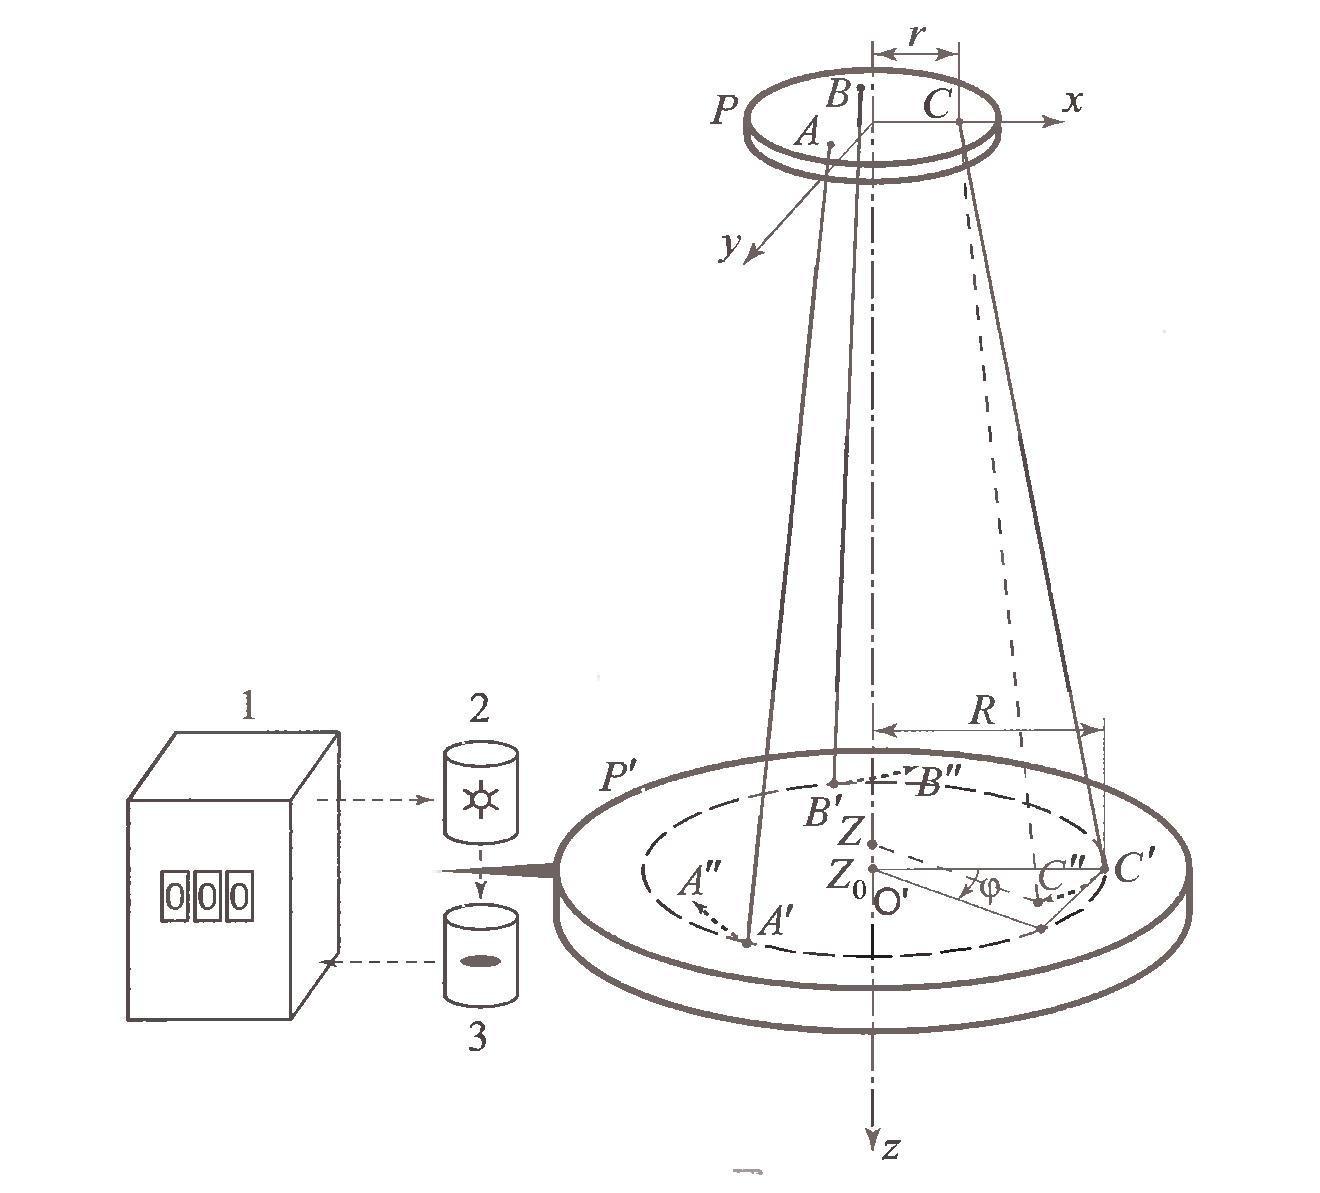
\includegraphics[width=0.95\linewidth]{1.2.3 ustan.png}
		\caption{Физический маятник}\label{risunok}
	\end{wrapfigure}

	Для наших целей удобно использовать устройство, показанное на Рис. \ref{risunok} и называемое трифилярным подвесом. Оно состоит из укрепленной на некоторой высоте неподвижной платформы $P$ и подвешенной к ней на трех симметрично расположенных нитях $AA'$, $BB'$ и $CC'$, вращающейся платформы $P'$.

	Чтобы не вызывать дополнительных раскачиваний, лучше поворачивать верхнюю платформу, укрепленную на неподвижной оси. После поворота верхняя платформа остается неподвижной в течение всего процесса колебаний. После того, как нижняя платформа $P'$ оказывается повернутой на угол $\varphi$ относительно верхней платформы $P$ возникает момент сил, стремящийся вернуть нижнюю платформу в положение равновесия, при котором относительный поворот платформ отсутствует. В результате платформа совершает крутильные колебания.

	\noindent где $k = \frac{gRr}{4\pi^2z_0}$ -- величина, постоянная для данной установки.

	\section{Оборудование}
	Трифилярный подвес, секундомер, счетчик числа колебаний, набор тел, момент инерции которых надлежит измерить (диск, стержень, полный цилиндр и другие).


\end{document}
